%% KnowFeat — EDBT 2027 Research Track (3rd Cycle) submission
%% Based on the official EDBT 2027 template (A4, sigconf+review, single-blind)
\documentclass[sigconf,review]{acmart}

%% A4 geometry override (copied from EDBT template)
\geometry{twoside=true, head=13pt,
     a4paper,
     includeheadfoot, columnsep=2pc,
     top=57pt, bottom=73pt, inner=54pt, outer=54pt,
     marginparwidth=2pc,heightrounded
     }%

\AtBeginMaketitle{%
  %% EDBT Conference Proceedings setup for ACM sigconf Style



%% EDBT: ISBN and year have to be adapted with every Number / Volume !
%%
\def\EDBTISSN{xxxx-xxxx}
\def\EDBTISBN{xxx-x-xxxxx-xxx-x}
\setcopyright{none}
\copyrightyear{\copyright\ 2027 Copyright held by the owner/author(s).
  Published on xxxxx under ISBN \EDBTISBN, series ISSN \EDBTISSN.
  Distribution of this paper is permitted under the terms of the
  Creative Commons license CC-by-nc-nd 4.0}
\acmYear{2027}
\acmDOI{}
\acmISBN{}


%% These commands are for a PROCEEDINGS abstract or paper.
%% EDBT: This needs adaptation every year!
\acmConference[EDBT '27]{Extending Database Technology}{6-9 April 2027}{Lille (France)}
%%
%%  Uncomment \acmBooktitle if the title of the proceedings is different
%%  from ``Proceedings of ...''!
%%
%%\acmBooktitle{Woodstock '18: ACM Symposium on Neural Gaze Detection,
%%  June 03--05, 2018, Woodstock, NY}


%% EDBT:
\settopmatter{printacmref=false, printccs=false, printfolios=false}


%% EDBT:
%% Macro to make image usable as hyperlink [see http://tex.stackexchange.com/questions/31819/xelatex-includegraphics-and-hyperlink]
\newsavebox{\ximagebox}
\newlength{\ximageheight}
\newsavebox{\xglyphbox}
\newlength{\xglyphheight}
\newcommand{\xbox}[1]%
  {\savebox{\ximagebox}{#1}%
  \settoheight{\ximageheight}{\usebox{\ximagebox}}%
  \savebox{\xglyphbox}{\color{white}\char32}%
  \settoheight{\xglyphheight}{\usebox{\xglyphbox}}%
  \raisebox{\ximageheight}[0pt][0pt]{\raisebox{-\xglyphheight}[0pt][0pt]{%
    \makebox[0pt][l]{\usebox{\xglyphbox}}}}%
    \usebox{\ximagebox}%
    \raisebox{0pt}[0pt][0pt]{\makebox[0pt][r]{\usebox{\xglyphbox}}}}

%% now use this to define the logo header:

\newsavebox{\LogoBox}
\sbox{\LogoBox}{}

%% now define our header and footer for the first page
\fancypagestyle{firstpagestyle}{%
  \fancyhf{}%
  \fancyfoot{}%
  \fancyhead[L,C]{}
  \fancyhead[R]{}{\raisebox{15pt}[0pt][0pt]{\xbox{\usebox{\LogoBox}}}}
  }

\hypersetup{%
  pdfcopyright={CC-by-nc-nd},
  pdfcreator={LaTeX with acmart, hyperref, and EDBT modifications},
  pdfvolumenum={XX},
  pdfissuenum={X},
  pdfisbn={\EDBTISBN},
  pdfissn={\EDBTISSN}
}

}% \AtBeginMaketitle

% Additional packages (acmart already loads amsmath, hyperref, booktabs, natbib)
% amssymb is NOT loaded by acmart but related_work.tex needs \checkmark.
\usepackage{amssymb}
\usepackage{algorithm}
% method.tex writes Algorithm 1 in algorithmic syntax (\STATE, \FOR, \TO),
% so load algorithmic here rather than algpseudocode.
\usepackage{algorithmic}
\usepackage{graphicx}
\usepackage{multirow}
\usepackage{placeins}
\usepackage{listings}

\lstset{
  basicstyle=\small\ttfamily,
  backgroundcolor=\color[gray]{0.95},
  frame=single,
  framerule=0pt,
  xleftmargin=3pt,
  xrightmargin=3pt,
  aboveskip=4pt,
  belowskip=4pt,
  columns=fullflexible,
  keepspaces=true,
  language=Python,
  keywordstyle=\small\ttfamily
}

\begin{document}
\emergencystretch=1.5em

\title{KnowFeat: Knowledge-Guided Feature Engineering via LLM Agents}

%% Single-blind: authors visible to reviewers
\author{Chengsong You}
\email{51275901122@stu.ecnu.edu.cn}
\affiliation{%
  \institution{East China Normal University}
  \city{Shanghai}
  \country{China}
}

\author{Wangyue Li}
\email{52285901017@stu.ecnu.edu.cn}
\affiliation{%
  \institution{East China Normal University}
  \city{Shanghai}
  \country{China}
}

\author{Weiqiao Que}
\email{weiqiaoque@gmail.com}
\affiliation{%
  \institution{East China Normal University}
  \city{Shanghai}
  \country{China}
}

\author{Qizhou Chen}
\email{582476065@qq.com}
\affiliation{%
  \institution{East China Normal University}
  \city{Shanghai}
  \country{China}
}

\author{Kunyan Wu}
\email{wky24@mails.tsinghua.edu.cn}
\affiliation{%
  \institution{Tsinghua University}
  \city{Beijing}
  \country{China}
}

\author{Feng Zhu}
\email{Jason_bank@126.com}
\affiliation{%
  \institution{Digital Currency Department, Postal Savings Bank of China}
  \city{Beijing}
  \country{China}
}

\author{Wei Deng}
\email{dengwei@swufe.edu.cn}
\affiliation{%
  \institution{Southwestern University of Finance and Economics}
  \city{Chengdu}
  \country{China}
}

\author{Xiaofeng He}
\email{hexf@cs.ecnu.edu.cn}
\affiliation{%
  \institution{East China Normal University}
  \city{Shanghai}
  \country{China}
}

\renewcommand{\shortauthors}{You et al.}

%% Abstract (abstract.tex contains \begin{abstract}...\end{abstract})
% abstract.tex
\begin{abstract}
Automated feature engineering with large language models (LLMs) can generate semantically meaningful features for tabular data, yet existing methods lack structured domain knowledge, rigorous verification, and auditable provenance. We propose \textbf{KnowFeat}, a knowledge-guided feature engineering framework that addresses all three gaps. KnowFeat organizes domain knowledge into a five-type hierarchy---schema metadata, regulatory indicators, detection rules, expert opinions, and case evidence---and injects it into an LLM agent. A three-stage verification pipeline (L1--L3) filters candidates through code execution, statistical quality checks, and model evaluation. Every accepted feature carries a provenance card tracing its design to specific knowledge assets. On seven public benchmarks, KnowFeat achieves the best AUC on 4 of 7 datasets and the best average rank (1.4) among seven methods. On a real-world anti-money laundering (AML) dataset with 200K transactions, 18 knowledge-guided features improve Recall by +2.1pp and F1 by +1.5pp over a 93-feature baseline, outperforming methods that generate up to 1{,}031 unverified features. Ablation studies confirm that hierarchical domain knowledge is essential for consistent feature quality.
\end{abstract}

\begin{IEEEkeywords}
Feature Engineering, Large Language Models, Domain Knowledge, Anti-Money Laundering, Tabular Data
\end{IEEEkeywords}


\keywords{Feature Engineering, Large Language Models, Domain Knowledge, Automated Feature Engineering, Anti-Money Laundering}

\maketitle

%% Body
% intro.tex
\section{Introduction}
\label{sec:intro}

Feature engineering is widely recognized as one of the most impactful steps in building machine learning models for tabular data~\cite{domingos2012few}. Carefully designed features can substantially improve model accuracy, reduce overfitting, and provide interpretable signals for downstream tasks. However, manual feature engineering is labor-intensive, requires deep domain expertise, and does not scale.

Traditional automated feature engineering (AutoFE) methods such as OpenFE~\cite{zhang2023openfe} and AutoFeat~\cite{horn2019autofeat} explore a predefined transformation space without understanding what features \emph{mean}. The emergence of large language models (LLMs) has enabled semantic feature generation: CAAFE~\cite{hollmann2023caafe}, FeatLLM~\cite{han2024featllm}, and LLM-FE~\cite{abhyankar2025llmfe} use LLMs to generate feature code from dataset descriptions. However, these methods share three fundamental limitations:

\textbf{(1) Lack of structured domain knowledge.}
Existing methods rely on the LLM's parametric knowledge, which may be outdated or incomplete for specialized domains. None organizes external knowledge into a hierarchical format for systematic injection, yet such structured knowledge is abundant in regulated domains like anti-money laundering (AML)~\cite{fatf2012recommendations,weber2019anti}.

\textbf{(2) Insufficient verification.}
CAAFE uses a logistic regression proxy, LLM-FE uses downstream accuracy without statistical filtering, and FeatLLM performs no model-based validation. None combines code execution, statistical quality filtering, and model evaluation into a unified pipeline.

\textbf{(3) Limited auditability.}
In regulated industries, features must be auditable---decision-makers need to understand \emph{why} a feature was created and \emph{what evidence} supports it. No existing method provides structured provenance tracing each feature to specific knowledge assets.

We propose \textbf{KnowFeat} (\textbf{Know}ledge-guided \textbf{Feat}ure engineering), a framework that addresses all three limitations:

\begin{itemize}
    \item \textbf{Hierarchical Knowledge Injection.} We organize domain knowledge into five types of increasing specificity---schema metadata, risk indicators, detection rules, expert opinions, and case evidence---and inject them as structured context into the LLM agent.

    \item \textbf{Three-Stage Verification Pipeline.} Each candidate passes through L1 (code execution sandbox), L2 (statistical quality with noise-calibrated thresholds), and L3 (model effectiveness via XGBoost across 5 seeds).

    \item \textbf{Auditable Provenance.} Every accepted feature carries a provenance card recording the knowledge assets, reasoning chain, computation steps, and verification results.
\end{itemize}

We evaluate KnowFeat on seven public benchmarks from OpenML and SimECNY, a real-world AML dataset with 200{,}000 digital currency transactions and 93 baseline features. Key findings:

\begin{itemize}
    \item On public datasets, KnowFeat achieves the best AUC on 4 of 7 datasets and the best average rank (1.4) among seven methods, with significantly fewer features than LLM-based alternatives.
    \item On SimECNY, 18 knowledge-guided features improve Recall by +2.1pp and F1 by +1.5pp over the 93-feature baseline, outperforming all baselines.
    \item Ablation confirms that domain knowledge is essential: the schema-only variant generates zero accepted features on one dataset.
\end{itemize}

% related_work.tex
\section{Related Work}
\label{sec:related}

% Framework figure - placed early so it appears at top of page 3
\begin{figure*}[!t]
    \centering
    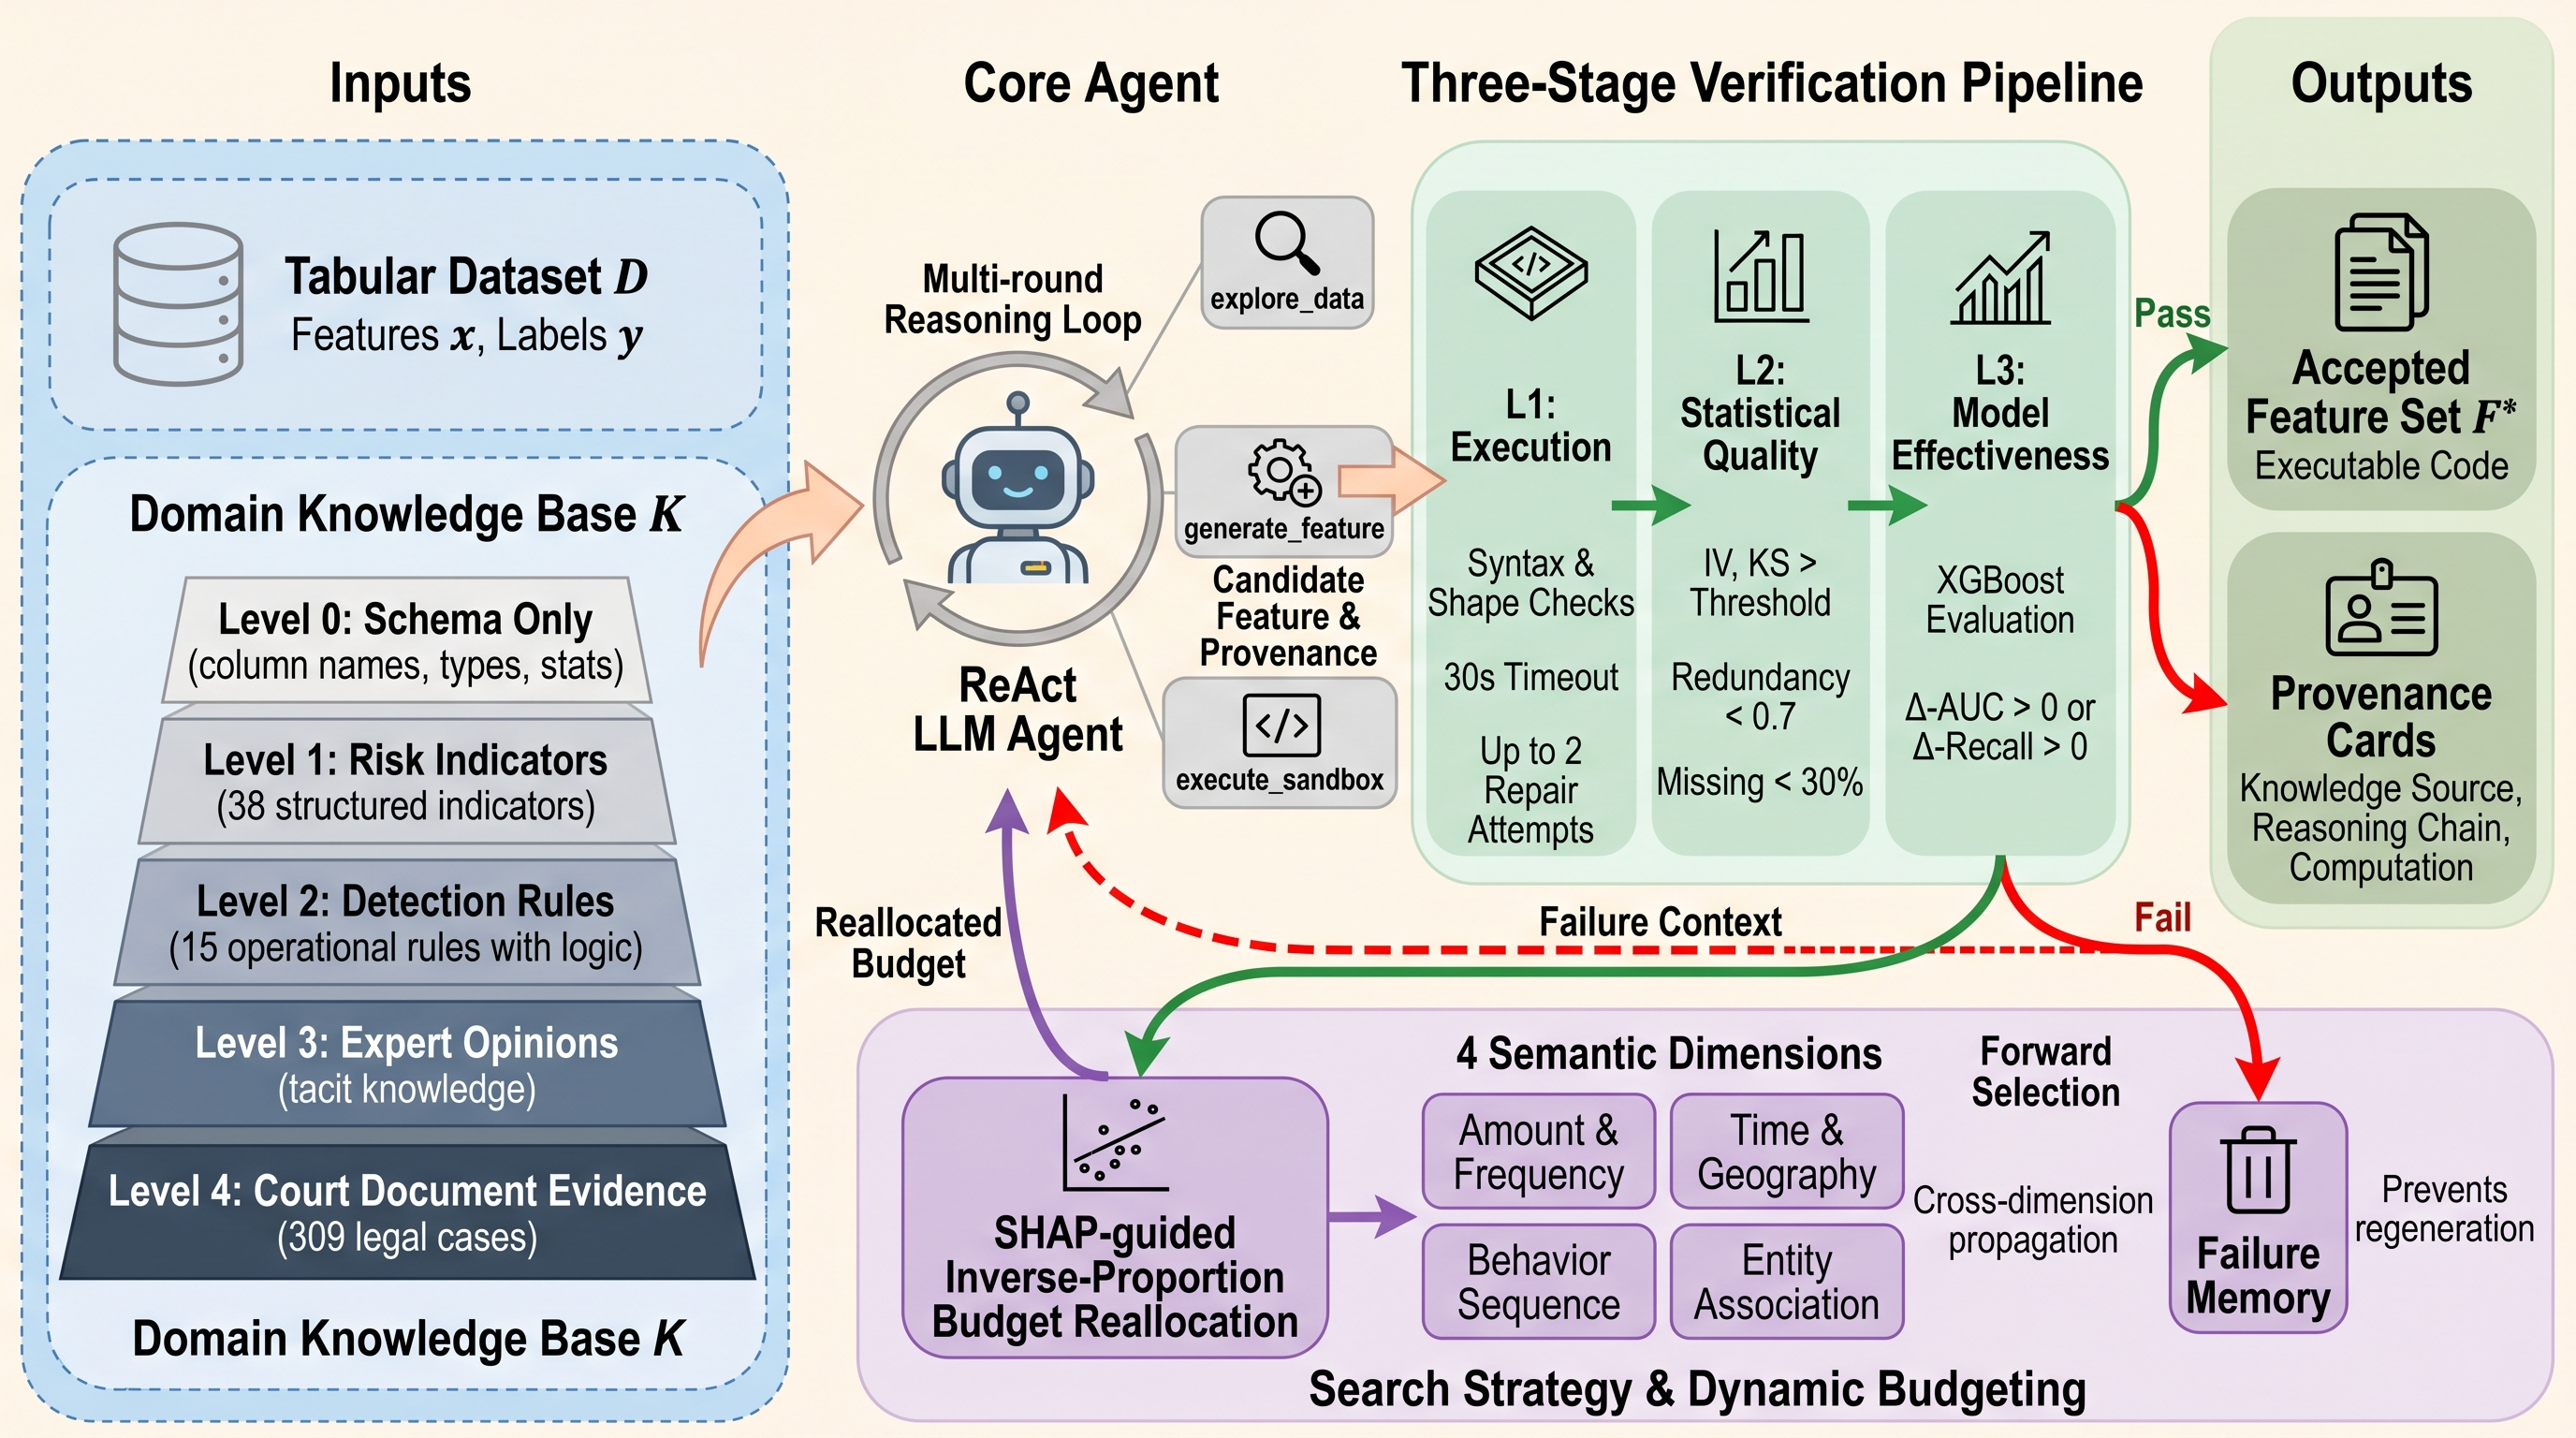
\includegraphics[width=0.85\textwidth]{figures/framework.png}
    \caption{Overview of the KnowFeat framework. Color coding: blue = inputs (data \& knowledge), yellow = core LLM agent, green = verification pipeline (L1--L3), purple = outputs (features \& provenance cards), gray = SHAP-guided search strategy. The agent generates features grounded in hierarchical domain knowledge; each candidate is verified through a three-stage pipeline; SHAP feedback dynamically reallocates the exploration budget across semantic dimensions.}
    \label{fig:framework}
\end{figure*}

\subsection{Automated Feature Engineering}

Traditional AutoFE methods search a \emph{syntactic} transformation space. Deep Feature Synthesis~\cite{kanter2015deep} applies aggregation primitives along relational paths; ExploreKit~\cite{katz2016explorekit} enumerates operators via meta-learning; AutoFeat~\cite{horn2019autofeat} uses polynomial expansion with L1 selection; and OpenFE~\cite{zhang2023openfe} frames generation as operator-operand search with LightGBM-based ranking. AutoML systems such as Auto-sklearn~\cite{feurer2015auto} and FLAML~\cite{wang2021flaml} include preprocessing but do not generate semantically new features. These methods apply predefined operators without \emph{semantic} understanding~\cite{nargesian2017learning}.

The emergence of LLMs~\cite{brown2020gpt3,touvron2023llama} enabled semantic feature generation. CAAFE~\cite{hollmann2023caafe} iteratively prompts an LLM to generate Python code using logistic regression feedback. FeatLLM~\cite{han2024featllm} extracts rules and converts them to binary indicators. LLM-FE~\cite{abhyankar2025llmfe} uses evolutionary optimization with model performance feedback. RiskTagger~\cite{li2025risktagger} uses regulatory knowledge for Web3 behavior annotation. Tool-augmented agents~\cite{yao2023react} have been applied to code generation~\cite{qian2024chatdev}, software engineering~\cite{jimenez2024swe}, and data science~\cite{hong2024data,jiang2025aide,guo2024ds}, but none addresses knowledge-grounded feature generation.

These methods vary in domain knowledge and verification depth. Table~\ref{tab:comparison} summarizes the key differences. KnowFeat is the first to combine hierarchical structured knowledge, multi-stage verification (L1--L3), and full provenance tracking.

In financial AML, domain experts manually encode risk indicators and network measures~\cite{chen2018aml}, regulatory bodies publish red-flag typologies~\cite{fatf2012recommendations}, and institutions maintain detection rules from compliance experience~\cite{weber2019anti}. Knowledge-infused learning~\cite{kursuncu2020knowledge} and transfer learning~\cite{weiss2016survey} target unstructured data rather than tabular features. This rich, structured AML knowledge has not been systematically leveraged by automated feature engineering.

\begin{table}[t]
\centering
\caption{Comparison of automated feature engineering methods. \checkmark: fully supported; $\circ$: partially supported; blank: not supported; --: not applicable.}
\label{tab:comparison}
\small
\renewcommand{\arraystretch}{1.2}
\setlength{\tabcolsep}{1pt}
\begin{tabular}{l c c c c c c c}
\hline
\textbf{Property} & \textbf{OpenFE} & \textbf{AutoF.} & \textbf{CAAFE} & \textbf{FeatL.} & \textbf{LLM-FE} & \textbf{RiskT.} & \textbf{Ours} \\
\hline
Semantic underst. &            &            & \checkmark & \checkmark & \checkmark & \checkmark & \checkmark \\
Hier.\ knowledge  &            &            &            &            & $\circ^1$    & $\circ^2$    & \checkmark \\
Exec.\ verific.   & --         & --         &            &            &            &            & \checkmark \\
Statistical filt. & \checkmark & \checkmark &            &            &            &            & \checkmark \\
Model validation  &            &            & $\circ^3$       &            & \checkmark &            & \checkmark \\
Provenance track. &            &            &            &            &            & $\circ^4$    & \checkmark \\
Adaptive search   &            &            &            &            & \checkmark &            & \checkmark \\
\hline
\multicolumn{8}{l}{\scriptsize $^1$Dataset desc.\ only. $^2$Regulatory guidelines only. $^3$LogReg proxy. $^4$NL rationales only.} \\
\end{tabular}
\end{table}

% method.tex
\section{Methodology}
\label{sec:method}

This section presents the KnowFeat framework in detail. We first provide an overview of the pipeline (Section~\ref{subsec:overview}), then describe each component: multi-type knowledge injection (Section~\ref{subsec:knowledge}), the LLM agent with specialized tools (Section~\ref{subsec:agent}), the three-stage verification pipeline (Section~\ref{subsec:verification}), the intelligent search strategy (Section~\ref{subsec:search}), and explainable provenance output (Section~\ref{subsec:provenance_method}).

\subsection{Framework Overview}
\label{subsec:overview}

KnowFeat is a multi-round, knowledge-guided feature engineering framework built on an LLM agent. Given a tabular dataset with baseline features and target labels, along with a domain knowledge base, KnowFeat generates a set of new features such that appending them to the original data improves predictive performance on a target metric (e.g., AUC or Recall).

The overall pipeline operates as follows (see Figure~\ref{fig:framework} for an illustration):

\begin{enumerate}
    \item \textbf{Initialization.} Load the dataset, compute baseline model performance, and calibrate statistical thresholds via noise injection (Section~\ref{subsec:verification}).
    \item \textbf{Knowledge Assembly.} Organize domain knowledge $\mathcal{K}$ into a five-type taxonomy and inject the selected types into the agent's context (Section~\ref{subsec:knowledge}).
    \item \textbf{Multi-Round Generation.} For each round $r = 1, \ldots, R_{\max}$:
    \begin{enumerate}
        \item Allocate per-dimension budgets based on SHAP feedback from the previous round.
        \item For each semantic dimension (Section~\ref{subsec:search}), the LLM agent explores the data, proposes candidate features grounded in knowledge assets, and submits them for verification.
        \item Each candidate passes through the L1$\to$L2$\to$L3 pipeline. Accepted features are added to the baseline; rejected features enter the failure memory.
        \item Forward selection discovers feature combinations that are individually weak but collectively effective.
    \end{enumerate}
    \item \textbf{Convergence.} The process terminates when no new features are accepted for $C$ consecutive rounds (default $C=2$) or the maximum round count $R_{\max}$ is reached.
    \item \textbf{Output.} The accepted feature set $\mathcal{F}^*$, along with executable code and explainable provenance cards for each feature (Section~\ref{subsec:provenance_method}).
\end{enumerate}

\subsection{Multi-Type Knowledge Injection}
\label{subsec:knowledge}

KnowFeat systematically integrates external domain knowledge into the feature generation process. We organize knowledge into five types of increasing specificity, from general metadata to concrete case evidence:

\textbf{(1) Schema Metadata.} The agent receives only the dataset schema: column names, data types, and basic statistics (mean, cardinality, missing rate). No domain knowledge is provided. This serves as the ablation baseline, testing what the LLM can generate from metadata alone.

\textbf{(2) Risk Indicators.} Structured risk indicators derived from regulatory guidelines and industry standards. Each indicator specifies a risk dimension, risk class, relevant data field, and directionality. For the AML domain, we compile 38 indicators (IND\_01 through IND\_38) covering transaction amount thresholds, frequency patterns, temporal anomalies, and network centrality measures. For example, IND\_05 flags accounts whose single-day transaction count exceeds a regulatory threshold, while IND\_15 identifies abnormal transaction modes such as fan-in and many-to-many patterns.

\textbf{(3) Detection Rules.} Operational detection rules that encode specific logic patterns. Each rule includes a rule ID, natural language description, logical expression, confidence level, and a Python implementation hint. We compile 15 rules (RULE\_001 through RULE\_015) from compliance manuals and internal documentation. For example, RULE\_006 encodes the ``scatter-in, gather-out'' layering pattern.

\textbf{(4) Expert Opinions.} Insights from domain expert interviews that capture tacit knowledge (heuristics, edge cases, and domain intuitions) difficult to formalize as rules but valuable for feature design. We collect 12 expert opinions (EXP\_01 through EXP\_12). For example, EXP\_05 notes that ``border region transactions combined with nighttime activity are a hallmark of cross-border laundering.''

\textbf{(5) Court Document Evidence.} Risk factors extracted from 309 real court judgments via a key-clue extraction pipeline. This is the most concrete type, grounding feature generation in case evidence (e.g., pyramid-shaped fund network patterns independently validated by legal proceedings).

The five types can be freely combined via a knowledge filter parameter, enabling ablation study of each type's contribution. In the ``full'' configuration (default), all types are included. Each knowledge item is assigned a unique identifier for provenance tracking.

\subsection{LLM Agent with Specialized Tools}
\label{subsec:agent}

KnowFeat employs an LLM agent (DeepSeek-V4-0324-Flash in our implementation, with temperature=0 for near-deterministic outputs) that interleaves reasoning with tool calls following the ReAct paradigm~\cite{yao2023react}. The agent is equipped with three specialized tools:

\textbf{Tool 1: Data Exploration.} Executes Python code on the dataset in a sandboxed environment to inspect distributions, compute correlations, and identify patterns before proposing features. The tool returns printed output or return values to the agent.

\textbf{Tool 2: Feature Registration.} Registers a candidate feature with mandatory provenance fields:
\begin{itemize}
    \item \texttt{feature\_name}: A descriptive identifier.
    \item \texttt{code}: Executable Python code that computes the feature from raw data.
    \item \texttt{explanation}: A natural language description of what the feature captures.
    \item \texttt{reasoning}: A structured chain linking knowledge assets to the feature design, formatted as ``Step $N$: Because [knowledge ID] indicates [insight], we compute [transformation]\ldots''
    \item \texttt{knowledge\_ids}: A list of specific knowledge asset identifiers (e.g., RULE\_001, IND\_05, EXP\_03) that inspired the feature.
    \item \texttt{computation\_steps}: Step-by-step description from raw fields to the final feature value.
    \item \texttt{data\_fields\_used}: The raw columns consumed by the feature.
\end{itemize}

\textbf{Tool 3: Verification Trigger.} Triggers the L1$\to$L2$\to$L3 verification pipeline on a registered feature and returns the result (accepted/rejected with detailed reasons). The agent must call Feature Registration followed immediately by Verification Trigger for each candidate; batch submission is prohibited to ensure tight feedback loops.

The agent's prompt instructs it to:
(1) reason about which knowledge assets are relevant to the current dimension and budget,
(2) explore the data to validate assumptions,
(3) propose a feature grounded in specific knowledge items, and
(4) submit it for verification and react to the feedback.

\subsection{Three-Stage Verification Pipeline}
\label{subsec:verification}

Each candidate feature passes through three progressively stricter verification stages:

\subsubsection{L1: Code Execution Sandbox}
The generated Python code is executed in an isolated sandbox with a 30-second timeout. L1 checks for:
\begin{itemize}
    \item Syntax and runtime errors.
    \item Output shape consistency (one value per sample).
    \item Presence of required identifier columns.
    \item Data type validity (numeric output).
\end{itemize}
If L1 fails, the agent receives the error message and is allowed up to 2 automatic repair attempts before the feature is permanently rejected.

\subsubsection{L2: Statistical Quality Filtering}
The feature's statistical properties are evaluated against automatically calibrated thresholds. To establish these thresholds for discriminative power, we generate $N_{\text{noise}} = 100$ random features (drawn from standard distributions), compute their quality metrics, and set the acceptance threshold at the $P_{\text{noise}}$-th percentile (default $P_{\text{noise}} = 95$). This ensures that accepted features are statistically better than random noise. L2 checks four criteria:
\begin{itemize}
    \item \textbf{Information Value (IV)}~\cite{chen2018aml}: Must exceed the noise-calibrated threshold, ensuring the feature has meaningful discriminative power between positive and negative classes.
    \item \textbf{Kolmogorov--Smirnov (KS) Statistic}~\cite{nargesian2017learning}: Must exceed the noise-calibrated threshold, measuring the maximum distributional separation between classes.
    \item \textbf{Redundancy}: Maximum absolute Pearson correlation with all existing accepted features must be below 0.7, preventing near-duplicate features from inflating the feature set.
    \item \textbf{Missing Rate}: The proportion of NaN values must be at most 50\%, ensuring sufficient coverage for model training.
\end{itemize}
The noise-calibrated thresholds apply to IV and KS; the redundancy and missing rate thresholds are fixed.

\subsubsection{L3: Model Effectiveness}
The feature is evaluated for its actual contribution to predictive performance. We train an XGBoost~\cite{chen2016xgboost} model on the baseline features augmented with the candidate feature, using stratified 80/20 train-test splits across 5 random seeds $\{42, 123, 456, 789, 2024\}$. The acceptance criterion depends on the task:
\begin{itemize}
    \item \textbf{Classification (public datasets)}: $\Delta\text{AUC} > 0$, i.e., the augmented model must achieve strictly higher AUC than the baseline.
    \item \textbf{AML detection}: $\Delta\text{Recall} > 0$ \emph{and} Precision $\geq 90\%$, ensuring that the feature improves detection without sacrificing precision.
\end{itemize}

The three-stage design is intentionally progressive: L1 is cheap (milliseconds), L2 is moderate (seconds), and L3 is expensive (minutes per feature). By filtering early, we avoid wasting computational resources on clearly defective candidates.

\subsection{Intelligent Search Strategy}
\label{subsec:search}

To systematically explore the feature space, KnowFeat employs a multi-component search strategy.

\textbf{Dimension-Based Budgeting.}
We decompose the feature space into $D$ semantic dimensions relevant to the target domain (default $D=4$ for the AML domain): Amount \& Frequency, covering monetary values and transaction counts; Time \& Geography, capturing temporal patterns and spatial distributions; Behavior Sequence, encoding sequential patterns in user actions; and Entity Association, derived from relationships between entities such as accounts and counterparties.

Each dimension receives an initial budget of $B_0$ candidates per round (default $B_0 = 3$). After each round, SHAP~\cite{lundberg2017shap} (SHapley Additive exPlanations) analysis is performed on the current model to estimate each dimension's contribution to predictions.

\textbf{SHAP-Guided Budget Reallocation.}
Let $s_j$ denote the mean absolute SHAP value for dimension $j$'s accepted features, $B_{\min}$ the minimum per-dimension budget (default 1), and $B_{\text{total}}$ the total budget for the round. We reallocate the budget for round $r{+}1$ using an \emph{inverse-SHAP weighting} strategy:
\begin{equation}
    B_j^{(r+1)} = B_{\min} + (B_{\text{total}} - D \cdot B_{\min}) \cdot \frac{1/s_j}{\sum_{j'=1}^{D} 1/s_{j'}}
\end{equation}
This ensures that underrepresented dimensions (those contributing least to the current model) receive more exploration budget, promoting balanced feature coverage.

\textbf{Failure Memory.}
A failure memory $\mathcal{M}_{\text{fail}}$ records all rejected features along with their rejection reasons. Before each generation step, the $K$ most recent failures for the current dimension (default $K=10$) are injected into the agent's prompt, preventing the regeneration of previously rejected ideas and guiding the agent toward novel directions.

\textbf{Forward Selection.}
Individual features may fail L3 yet contribute positively when combined with others. We apply greedy forward selection on L2-passed but L3-failed candidates, sorted by L2 quality scores. Each candidate is added to the accepted set if the augmented set improves the target metric, capturing synergistic feature interactions.

\textbf{Cross-Dimension Propagation.}
After each round, the top-$K_{\text{cross}}$ features (default $K_{\text{cross}} = 5$) by SHAP importance are shared across all dimensions as ``inspiration prompts,'' encouraging the agent to adapt successful patterns from one dimension to others.

\subsection{Explainable Provenance Output}
\label{subsec:provenance_method}

Every generated feature is accompanied by a structured \emph{provenance card} that enables full explainability. Each provenance card records:
\begin{itemize}
    \item \textbf{Knowledge assets}: The specific identifiers (e.g., RULE\_006, IND\_15, EXP\_05) that inspired the feature design.
    \item \textbf{Reasoning chain}: A step-by-step explanation of how domain knowledge led to the feature, formatted as ``Step $N$: Because [knowledge ID] indicates [insight], we compute [transformation]\ldots''
    \item \textbf{Computation steps}: The transformation pipeline from raw data fields to the final feature value.
    \item \textbf{Verification results}: L1/L2/L3 outcomes including IV, KS, redundancy, and $\Delta$AUC/$\Delta$Recall.
\end{itemize}
This traceability is essential for regulated domains: compliance officers can trace \emph{why} each feature exists, \emph{what evidence} supports it, and \emph{how} it was verified. Section~\ref{sec:case_study} illustrates provenance cards through concrete examples.

% experiments.tex
\section{Experiments}
\label{sec:experiments}

We evaluate KnowFeat on both public tabular benchmarks and a real-world anti-money laundering (AML) dataset. Our experiments aim to answer four research questions:
\begin{itemize}
    \item \textbf{RQ1}: Does KnowFeat improve predictive performance on public datasets?
    \item \textbf{RQ2}: How does KnowFeat perform on a real-world AML task with severe class imbalance?
    \item \textbf{RQ3}: What is the contribution of domain knowledge? (Ablation study)
    \item \textbf{RQ4}: How does KnowFeat balance feature quantity vs.\ quality?
\end{itemize}

\subsection{Experimental Setup}
\label{subsec:setup}

\subsubsection{Datasets}
We use eight datasets summarized in Table~\ref{tab:datasets}: seven public benchmarks from OpenML and one real-world AML dataset.

\begin{table}[t]
\centering
\caption{Dataset statistics.}
\label{tab:datasets}
\small
\renewcommand{\arraystretch}{1.2}
\setlength{\tabcolsep}{3pt}
\begin{tabular}{l r r r l}
\hline
\textbf{Dataset} & \textbf{Samples} & \textbf{Feat.} & \textbf{Pos\%} & \textbf{Domain} \\
\hline
credit\_g          & 1,000   & 20  & 70.0 & Finance \\
diabetes           & 768     & 8   & 34.9 & Healthcare \\
blood\_transfusion & 748     & 4   & 23.8 & Healthcare \\
heart              & 918     & 11  & 55.3 & Healthcare \\
bank\_marketing    & 45,211  & 16  & 11.7 & Marketing \\
breast\_w          & 683     & 9   & 35.0 & Healthcare \\
adult              & 48,842  & 14  & 23.9 & Census \\
SimECNY (AML)      & 200,000 & 93  & 2.24 & Finance \\
\hline
\end{tabular}
\end{table}

The seven public datasets are standard tabular benchmarks covering diverse domains. SimECNY is a real-world digital currency transaction dataset containing 200,000 transactions with 93 baseline features and 4,484 positive (suspicious) samples, representing a realistic AML scenario with severe class imbalance (2.24\% positive rate).

\subsubsection{Baselines}
We compare against five baselines:
\begin{itemize}
    \item \textbf{No-FE}: XGBoost on original features.
    \item \textbf{OpenFE}~\cite{zhang2024openfe}: Transformation-based AutoFE with LightGBM-based selection.
    \item \textbf{AutoFeat}~\cite{horn2020set}: Polynomial feature generation with L1 selection.
    \item \textbf{CAAFE}~\cite{hollmann2024llmsgeneratefinanciallyrelevantfeatures}: LLM-based iterative feature generation.
    \item \textbf{FeatLLM}~\cite{han2024featllm}: LLM-based rule extraction and binary feature generation.
\end{itemize}

\subsubsection{Evaluation Protocol}
All methods are evaluated using XGBoost (n\_estimators=200, max\_depth=6, learning\_rate=0.1) with stratified 80/20 train-test splits across 5 random seeds. For public datasets, the primary metric is AUC. For SimECNY, we report Recall, Precision, F1, and AUC with scale\_pos\_weight=auto ($\approx$43.6) to handle class imbalance. We additionally evaluate with scale\_pos\_weight=1 (no class balancing) to isolate the intrinsic quality of generated features.

\subsection{RQ1: Public Dataset Performance}
\label{subsec:rq1}

Table~\ref{tab:main_results} presents the AUC comparison on seven public datasets. KnowFeat achieves the best performance on 4 out of 7 datasets (credit\_g, blood\_transfusion, breast\_w, and adult) and ranks second on 2 datasets (diabetes and heart).

\begin{table*}[t]
\centering
\caption{AUC comparison on public datasets (mean$\pm$std over 5 seeds). \textbf{Bold}: best; \underline{underline}: second best. T/O = timeout.}
\label{tab:main_results}
\small
\renewcommand{\arraystretch}{1.2}
\setlength{\tabcolsep}{6pt}
\begin{tabular}{l c c c c c c}
\hline
\textbf{Dataset} & \textbf{No-FE} & \textbf{OpenFE} & \textbf{AutoFeat} & \textbf{CAAFE} & \textbf{FeatLLM} & \textbf{KnowFeat} \\
\hline
credit\_g          & .7670{\scriptsize$\pm$.021} & \underline{.7833{\scriptsize$\pm$.031}} & .7540{\scriptsize$\pm$.017} & .7596{\scriptsize$\pm$.023} & .7604{\scriptsize$\pm$.022} & \textbf{.7854{\scriptsize$\pm$.014}} \\
diabetes           & .8027{\scriptsize$\pm$.033} & \textbf{.8252{\scriptsize$\pm$.034}} & .8089{\scriptsize$\pm$.027} & .8032{\scriptsize$\pm$.030} & .8096{\scriptsize$\pm$.032} & \underline{.8190{\scriptsize$\pm$.032}} \\
blood\_transfusion & .6824{\scriptsize$\pm$.043} & .6654{\scriptsize$\pm$.040} & .6824{\scriptsize$\pm$.043} & .6779{\scriptsize$\pm$.043} & .6805{\scriptsize$\pm$.044} & \textbf{.7007{\scriptsize$\pm$.036}} \\
heart              & .9320{\scriptsize$\pm$.007} & \textbf{.9417{\scriptsize$\pm$.011}} & .9340{\scriptsize$\pm$.003} & .9302{\scriptsize$\pm$.006} & .9297{\scriptsize$\pm$.004} & \underline{.9379{\scriptsize$\pm$.006}} \\
bank\_marketing    & .9330{\scriptsize$\pm$.002} & \textbf{.9374{\scriptsize$\pm$.002}} & T/O & .9334{\scriptsize$\pm$.002} & .9337{\scriptsize$\pm$.002} & \underline{.9344{\scriptsize$\pm$.002}} \\
breast\_w          & .9926{\scriptsize$\pm$.005} & \underline{.9944{\scriptsize$\pm$.005}} & .9936{\scriptsize$\pm$.004} & .9924{\scriptsize$\pm$.006} & .9924{\scriptsize$\pm$.005} & \textbf{.9957{\scriptsize$\pm$.003}} \\
adult              & .9288{\scriptsize$\pm$.004} & \underline{.9300{\scriptsize$\pm$.003}} & .9254{\scriptsize$\pm$.004} & .9286{\scriptsize$\pm$.003} & .9289{\scriptsize$\pm$.003} & \textbf{.9301{\scriptsize$\pm$.003}} \\
\hline
\textbf{Avg.\ Rank} & 4.1 & \underline{2.1} & 4.4 & 4.9 & 4.1 & \textbf{1.4} \\
\hline
\end{tabular}
\end{table*}

KnowFeat achieves the best average rank (1.4), outperforming OpenFE (2.1). The largest improvements occur on datasets where domain knowledge provides strong semantic guidance: credit\_g (+0.018 over No-FE) and blood\_transfusion (+0.018 over No-FE).

OpenFE achieves the best results on 3 datasets (diabetes, heart, bank\_marketing) through exhaustive operator-operand search. However, OpenFE generates 34--50 features per dataset, while KnowFeat achieves competitive or superior performance with 12--46 features (see Section~\ref{subsec:rq4}).

CAAFE and FeatLLM perform close to the No-FE baseline on most datasets, suggesting that features generated without rigorous verification often introduce noise rather than signal.

\subsection{RQ2: AML Dataset Performance}
\label{subsec:rq2}

Table~\ref{tab:simecny} presents results on the SimECNY AML dataset with scale\_pos\_weight=auto. KnowFeat adds 18 knowledge-guided features to the 93-feature baseline, achieving the best results across all four metrics.

\begin{table}[t]
\centering
\caption{SimECNY AML results (spw=auto, 5 seeds).}
\label{tab:simecny}
\small
\renewcommand{\arraystretch}{1.2}
\setlength{\tabcolsep}{2pt}
\begin{tabular}{l r c c c c}
\hline
\textbf{Method} & $\boldsymbol{n_f}$ & \textbf{Recall} & \textbf{Prec.} & \textbf{F1} & \textbf{AUC} \\
\hline
No-FE     & 93   & .9663{\scriptsize$\pm$.010} & .9764{\scriptsize$\pm$.004} & .9713{\scriptsize$\pm$.005} & .9996 \\
OpenFE    & 123  & .9645{\scriptsize$\pm$.008} & .9752{\scriptsize$\pm$.004} & .9698{\scriptsize$\pm$.003} & .9996 \\
CAAFE     & 94   & .9681{\scriptsize$\pm$.008} & .9725{\scriptsize$\pm$.006} & .9703{\scriptsize$\pm$.005} & .9996 \\
FeatLLM   & 1124 & .9625{\scriptsize$\pm$.010} & .9728{\scriptsize$\pm$.005} & .9676{\scriptsize$\pm$.006} & .9995 \\
\textbf{Ours} & \textbf{111} & \textbf{.9871}{\scriptsize$\pm$.006} & \textbf{.9855}{\scriptsize$\pm$.001} & \textbf{.9863}{\scriptsize$\pm$.003} & \textbf{.9999} \\
\hline
\end{tabular}
\end{table}

KnowFeat's 18 domain-knowledge features yield substantial improvements: Recall improves by +2.1pp over No-FE (0.9871 vs.\ 0.9663), F1 by +1.5pp (0.9863 vs.\ 0.9713), and AUC reaches 0.9999. In contrast, OpenFE adds 30 features yet \emph{decreases} Recall, while FeatLLM adds 1,031 features and achieves the \emph{worst} performance across all metrics. This demonstrates that knowledge-guided features provide qualitatively different signal from syntactic transformations.

\subsubsection{Robustness Analysis (spw=1)}

To verify that KnowFeat's gains stem from intrinsic feature quality rather than interaction with class balancing, we re-evaluate all methods with scale\_pos\_weight=1 (Table~\ref{tab:simecny_spw1}).

\begin{table}[t]
\centering
\caption{SimECNY AML results (spw=1, 5 seeds).}
\label{tab:simecny_spw1}
\small
\renewcommand{\arraystretch}{1.2}
\setlength{\tabcolsep}{2pt}
\begin{tabular}{l r c c c c}
\hline
\textbf{Method} & $\boldsymbol{n_f}$ & \textbf{Recall} & \textbf{Prec.} & \textbf{F1} & \textbf{AUC} \\
\hline
No-FE     & 93   & .9409{\scriptsize$\pm$.011} & .9934{\scriptsize$\pm$.002} & .9664{\scriptsize$\pm$.006} & .9996 \\
OpenFE    & 123  & .9342{\scriptsize$\pm$.012} & .9912{\scriptsize$\pm$.002} & .9619{\scriptsize$\pm$.007} & .9995 \\
CAAFE     & 94   & .9382{\scriptsize$\pm$.012} & .9922{\scriptsize$\pm$.002} & .9644{\scriptsize$\pm$.007} & .9996 \\
FeatLLM   & 1124 & .9298{\scriptsize$\pm$.014} & .9912{\scriptsize$\pm$.002} & .9595{\scriptsize$\pm$.008} & .9995 \\
\textbf{Ours} & \textbf{111} & \textbf{.9683}{\scriptsize$\pm$.010} & \textbf{.9945}{\scriptsize$\pm$.004} & \textbf{.9812}{\scriptsize$\pm$.005} & \textbf{.9999} \\
\hline
\end{tabular}
\end{table}

Without class balancing, KnowFeat remains the clear winner, with Recall 0.9683 (+2.7pp over No-FE) and F1 0.9812 (+1.5pp). Importantly, KnowFeat is the \emph{only} method that outperforms the No-FE baseline---all other feature engineering methods \emph{degrade} Recall relative to the 93-feature baseline. Moreover, KnowFeat suffers the smallest Recall drop when switching from spw=auto to spw=1 ($\Delta = -$1.9pp), while FeatLLM drops the most ($\Delta = -$3.3pp). This confirms that KnowFeat's 18 features encode genuine discriminative signal that does not depend on class reweighting.

\subsection{RQ3: Ablation Study}
\label{subsec:rq3}

To quantify the contribution of domain knowledge, we compare the \textit{schema\_only} variant (Level 0: only dataset metadata) against the \textit{full} variant (all knowledge levels). Results on public datasets are shown in Table~\ref{tab:ablation}.

\begin{table}[t]
\centering
\caption{Ablation: schema\_only vs.\ full KnowFeat (AUC).}
\label{tab:ablation}
\small
\renewcommand{\arraystretch}{1.2}
\setlength{\tabcolsep}{3pt}
\begin{tabular}{l c c c}
\hline
\textbf{Dataset} & \textbf{schema\_only} & \textbf{full} & $\boldsymbol{\Delta}$ \\
\hline
credit\_g     & .7750{\scriptsize$\pm$.012} & \textbf{.7854}{\scriptsize$\pm$.014} & +.010 \\
blood\_trans.  & .6891{\scriptsize$\pm$.048} & \textbf{.7007}{\scriptsize$\pm$.036} & +.012 \\
heart         & .9304{\scriptsize$\pm$.005} & \textbf{.9379}{\scriptsize$\pm$.006} & +.008 \\
bank\_mkt.    & .9314{\scriptsize$\pm$.002} & \textbf{.9344}{\scriptsize$\pm$.002} & +.003 \\
adult         & .9292{\scriptsize$\pm$.003} & \textbf{.9301}{\scriptsize$\pm$.003} & +.001 \\
breast\_w     & \textbf{.9964}{\scriptsize$\pm$.002} & .9957{\scriptsize$\pm$.003} & $-$.001 \\
diabetes      & --- (0 feat.) & .8190{\scriptsize$\pm$.032} & --- \\
\hline
\end{tabular}
\end{table}

\textbf{Knowledge drives feature generation.} On the diabetes dataset, the schema-only variant generates \emph{zero} features that pass L3 verification---the LLM cannot create useful features from column names alone. With full knowledge, KnowFeat generates 24 accepted features and improves AUC by +0.016 over No-FE.

\textbf{Knowledge improves feature quality.} On five of the six remaining datasets, the full variant outperforms schema\_only, with gains ranging from +0.001 (adult) to +0.012 (blood\_transfusion). On blood\_transfusion, both variants generate 12 features, indicating that the improvement comes from feature \emph{quality}---domain knowledge guides the agent toward more predictive transformations.

\textbf{breast\_w exception.} On breast\_w, schema\_only slightly outperforms full ($-$0.001 AUC). We attribute this to the near-ceiling baseline (AUC $>$ 0.99), where additional features may introduce marginal noise.

\subsection{RQ4: Feature Quantity vs.\ Quality}
\label{subsec:rq4}

Table~\ref{tab:feature_count} compares the number of features generated by each method.

\begin{table}[t]
\centering
\caption{Number of features (incl.\ original).}
\label{tab:feature_count}
\small
\renewcommand{\arraystretch}{1.2}
\setlength{\tabcolsep}{2.5pt}
\begin{tabular}{l r r r r r r}
\hline
\textbf{Dataset} & \textbf{No-FE} & \textbf{OpenFE} & \textbf{Auto.} & \textbf{CAAFE} & \textbf{Feat.} & \textbf{Ours} \\
\hline
credit\_g     & 20  & 50  & 23  & 24  & 280  & 46  \\
diabetes      & 8   & 38  & 13  & 9   & 152  & 24  \\
blood\_trans. & 4   & 34  & 4   & 7   & 120  & 12  \\
heart         & 11  & 41  & 21  & 14  & 98   & 31  \\
bank\_mkt.    & 16  & 46  & T/O & 21  & 132  & 36  \\
breast\_w     & 9   & 39  & 20  & 10  & 107  & 16  \\
adult         & 14  & 44  & 165 & 19  & 170  & 34  \\
SimECNY       & 93  & 123 & --- & 94  & 1124 & 111 \\
\hline
\end{tabular}
\end{table}

FeatLLM generates by far the most features (98--1,124) yet achieves the worst or near-worst performance on most datasets. This confirms that \emph{more features $\neq$ better performance} when verification is absent. AutoFeat generates 165 features on adult yet ranks last among all methods (AUC 0.9254), further illustrating this point.

KnowFeat strikes an effective balance: it generates a moderate number of features (12--46 on public datasets, +18 on SimECNY) that have all passed the L1$\to$L2$\to$L3 pipeline. On SimECNY, the contrast is particularly stark: KnowFeat's 18 verified features improve F1 by +1.5pp, while FeatLLM's 1,031 unverified features \emph{decrease} F1 by $-$0.4pp. This demonstrates the effectiveness of quality-over-quantity feature engineering.

\subsection{Provenance and Interpretability}
\label{subsec:provenance}

Every KnowFeat-generated feature includes a provenance card recording: (1) the knowledge assets that inspired it; (2) a reasoning chain explaining \emph{why} the feature is relevant; and (3) the computation steps from raw fields to the final value. This traceability is essential for deployment in regulated industries. We illustrate this capability through detailed case studies in Section~\ref{sec:case_study}.

% conclusion.tex
\section{Conclusion}
\label{sec:conclusion}

We presented KnowFeat, a knowledge-guided feature engineering framework that combines hierarchical domain knowledge injection, multi-stage verification (L1--L3), and intelligent search strategies within an LLM agent. On seven public datasets, KnowFeat achieves the best AUC on 4 out of 7 and the best average rank (1.4) among all methods, while generating 3--10$\times$ fewer features than FeatLLM. On a real-world AML dataset with 200K transactions, 18 knowledge-guided features improve Recall by +2.1pp and F1 by +1.5pp over a strong 93-feature baseline---gains that are robust across different class balancing settings. The ablation study confirms that domain knowledge is essential, and every generated feature is traceable to specific knowledge assets.

\textbf{Limitations and Future Work.}
First, our current knowledge hierarchy is manually organized; automating knowledge extraction from heterogeneous sources (regulations, case law, expert interviews) is a promising direction.
Second, KnowFeat currently uses a single LLM; a multi-agent architecture with specialized agents for knowledge retrieval, feature proposal, and verification could improve efficiency.
Third, extending KnowFeat to additional high-stakes domains such as cybersecurity and insurance fraud detection would validate the generality of the approach.
Finally, investigating adaptive L3 thresholds to balance feature quantity and quality across different dataset characteristics is an important direction.


%% Artifacts section (required by EDBT before references)
\section*{Artifacts}
The source code and all datasets used in this paper are publicly available.
The code repository is at \url{https://github.com/youchengsong/large-llm-create-feature}.
The SimECNY dataset and public dataset knowledge bases are available at \url{https://huggingface.co/datasets/anonymous-7219/knowfeat}.

%% References
\balance
\bibliographystyle{ACM-Reference-Format}
\bibliography{references}

%% Appendix (appendix.tex contains \appendix command)
% appendix.tex
\appendix

\section{Domain Knowledge Examples for the AML Dataset}
\label{sec:appendix_knowledge}

This appendix illustrates the five knowledge types provided to KnowFeat for the SimECNY anti-money laundering dataset ($\sim$200K digital yuan transactions). One representative example per type is shown.

\smallskip
\noindent\textbf{(i) Schema Metadata.}
Column names, data types, and basic statistics extracted directly from the transaction data. No external knowledge is provided. Example fields: \texttt{amount} (numeric, mean=2{,}847.3), \texttt{wallet\_type} (categorical, 4 types), \texttt{hour} (numeric, 0--23), \texttt{src}/\texttt{dst} (account identifiers).

\smallskip
\noindent\textbf{(ii) Risk Indicator.}
\begin{quote}
\small
\textbf{IND\_05 -- Single-Day Transaction Frequency.} Field: \texttt{timestamp}, \texttt{src}. Direction: higher daily count increases risk. Threshold: $\geq$10 transactions/day triggers alert. Rationale: money mule accounts exhibit abnormally high transaction frequency to rapidly channel funds before detection; regulatory guidelines flag accounts exceeding normal daily activity levels.
\end{quote}

\smallskip
\noindent\textbf{(iii) Detection Rule.}
\begin{quote}
\small
\textbf{RULE\_006 -- Scatter-In, Gather-Out Layering.} Fields: \texttt{src}, \texttt{dst}, \texttt{amount}, \texttt{timestamp}. Logic: an account receives funds from $\geq$5 distinct sources within 24h AND transfers $\geq$80\% of cumulative amount to $\leq$2 destinations within 48h. This rule captures the classic ``fan-in, fan-out'' layering pattern where illicit funds are aggregated and rapidly consolidated.
\end{quote}

\smallskip
\noindent\textbf{(iv) Expert Opinion.}
\begin{quote}
\small
\textbf{EXP\_05.} Border-region transactions combined with nighttime activity (00:00--06:00) are a hallmark of cross-border laundering via digital yuan. Feature engineering should construct a \texttt{night\_border\_risk} interaction feature combining geographic indicators with temporal concentration.
\end{quote}

\smallskip
\noindent\textbf{(v) Court Document Evidence.}
\begin{quote}
\small
\textbf{CASE\_038 -- Pyramid-Shaped Fund Network.} Source: court judgment on digital yuan money laundering. Pattern: the defendant used multiple bank wallets (across 6 banks) to create a multi-layer fund channeling network, receiving funds from upstream accounts and immediately dispersing them via digital yuan transfers. Observable signals: funds traverse $\geq$3 layers within 24h; each layer address is active for $<$48h.
\end{quote}


\end{document}
